\section{Introduction}
\label{sc:introduction}


% Opening paragraph and the need for hardware solutions
In recent years, there has been considerable interest in \glspl{RIS}, particularly within the context of 6G communications.  The potential for significant improvements in communication and sensing capabilities through the use of large, passive, and tunable reflectors has led to the development of theoretical models and algorithms in the wireless communication community \cite{di2020smart,yu2021smart} and subsequent attention from the microwave community towards the practical implementation of \glspl{RIS}~\cite{kazim2020wireless}.

% What is a RIS and typical scenario for improving the wireless channel
\glspl{RIS} are planar electromagnetic surfaces comprised of many independently tunable reflecting elements. 
These reflecting elements can be adjusted externally to modify the phase and, in certain instances, the amplitude of the signal reflected at each element. % \red{\cite{venkatesh2022programmable}}. 
Through the superposition of reflections from each element, the reflection pattern can be dynamically tuned, eliminating the need for complex decoding, encoding, and processing. 
While demonstrations of reflectarrays and predictions on its tunability date back to 1963 \cite{berry1963reflectarray}, their large-scale application to mobile networks (see Fig.~\ref{fig:RISScenario}) has only been recently considered.

\begin{figure}[t]
	\centering
	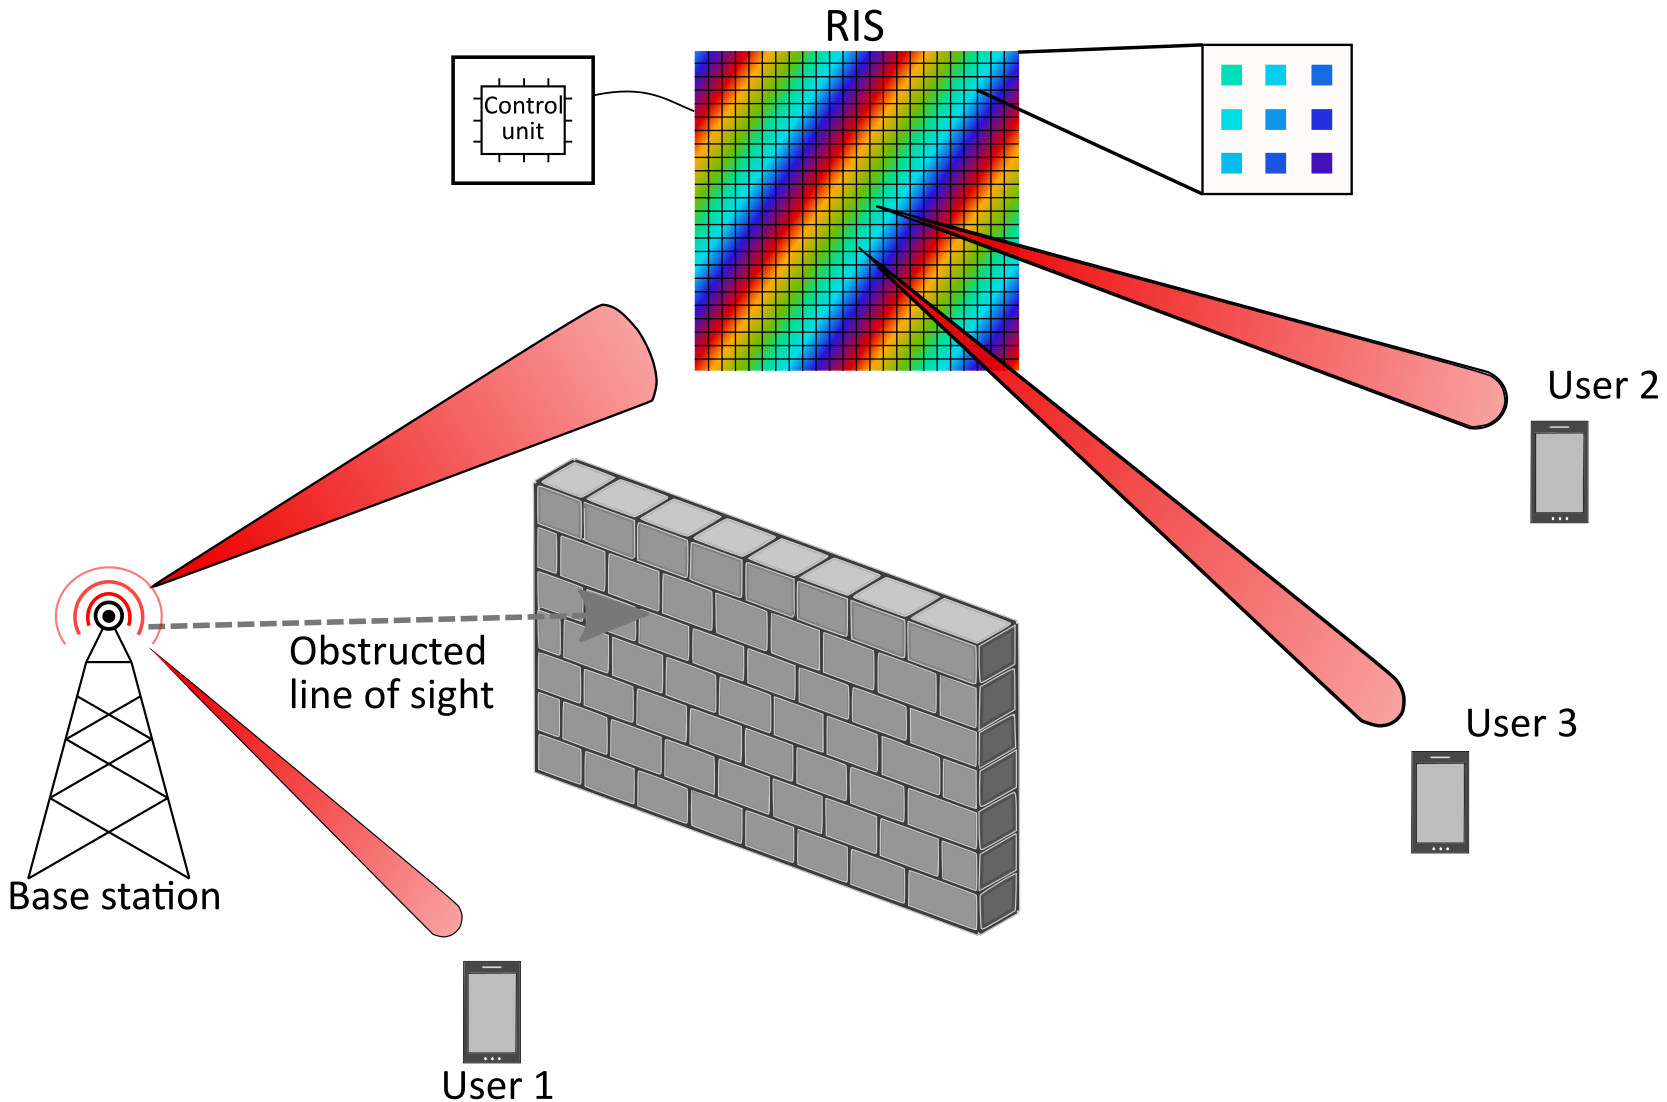
\includegraphics[width=0.96\columnwidth]{Figures/Motivation.png}
	\caption{Example scenario where a \gls{RIS} establishes a link between a transmitter and two receivers despite an obstacle blocking the \gls{LOS} path.}
	\label{fig:RISScenario}
\end{figure}

% Introducing LC crystals
    So far, various \gls{RIS} prototypes have been reported in the literature, which mainly employ \gls{SC} technologies (e.g., \gls{PIN} diodes \cite{tang2020wireless}, varactors \cite{alamzadeh2021reconfigurable}, % conference
    \gls{RF} switches \cite{rossanese2022designing}) to realize the phase shifts. Although a feasible choice of design, their cost and resolution (in case of \gls{PIN} diodes) can be prohibitive in building truly large and cost-efficient large \glspl{RIS}. An alternative to these technologies is \gls{NLC} technology. In the last two decades, \glspl{NLC} have been studied for the microwave, \gls{mm-Wave}, and THz frequency bands \cite[Ch. 5]{ferrari2022reconfigurable}. %\red{\cite{weickhmann2017liquid}}. 
    If fabrication in standard \gls{LCD} technology is adopted, the manufacturing cost of \gls{NLC}-\glspl{RIS} will be reduced to that of a commercial \gls{LCD} television. Hence, \gls{NLC}-based designs have the advantages of cost-effective scalability, low energy consumption, and continuous phase shifting, which make them a suitable candidate for realizing extremely large passive \glspl{RIS}. Despite these attractive features, \gls{NLC} characteristics impose new challenges when being integrated into today's mobile communication systems, most notably due to their slow tuning capabilities as compared with \gls{SC}-\glspl{RIS}.

% Contributions of this paper:
In this article, we aim at bridging the gap between microwave and antenna design aspects of \gls{NLC}-\glspl{RIS} with mobile communication aspects. To this end, we first review the basic physical principles of LC theory and introduce two different realizations of \gls{NLC}-\glspl{RIS}, namely the \gls{RA} and \gls{PA} methods. Thereby, we particularly highlight their key physical and hardware properties that have a direct impact on the system design and RIS reconfiguration strategy. This is complemented by a concrete comparison against the alternative technologies for building RISs (i.e., \glspl{SC} and \gls{MEMS})  in terms of feasibility, cost, power consumption, reconfiguration speed, and bandwidth. Finally, we delve into the challenges of \gls{NLC}-\glspl{RIS} (slow response time, temperature dependencies, bandwidth) and present potential directions for both theoretical and experimental research in order to overcome these challenges.




% Basic path loss and phase gradients needed assuming far-field ozdogan2019intelligent

% \begin{itemize}
%     \item RISs have been the subject of extensive investigations in the past few years, esp in the context of 6G communications. 
%     \item then what are RISs... 
%     \item advantage and disadvantage --> Perhaps the cost and HW complexity can be listed as a disadvantage. --> This puts their practicality under question. and determines whether they will be used as a widely deployed technology or as a specialized high-end gadget limited to a few use cases.  
%     \item in this article, we provide an overview on what is the state of the art on RIS design. Bringing together the knowledge from antenna design and communication systems, we shed light on alternative technologies which allow scalable and effective RIS manufacturing and operations. 
% \end{itemize}

% Introduction

% In recent years, there has been considerable interest in \glspl{RIS}, particularly within the context of 6G communications. 
% The potential for significant improvements in communication and sensing capabilities through the use of large, passive tunable reflectors has led to the development of models and subsequent attention from the microwave community towards the practical implementation of \glspl{RIS}~\cite{kazim2020wireless}.

% \glspl{RIS} have been the subject of extensive investigations in the past few years, especially in the context of 6G communications. With the development of models predicting massive communication and sensing improvements through large, passive (from the \gls{RF} perspective) tunable reflectors, the attention of the \gls{RF} community has been brought towards the realization of such \glspl{RIS} }. 
%Tests include the enhancement of the wireless communications in rich scattering channels \cite{alexandropoulos2021reconfigurable}. % Missing some additional sentence

% What is a RIS and typical scenario
% \glspl{RIS} are planar electromagnetic surfaces comprised of many independently tunable reflecting elements. 
% These reflecting elements can be adjusted externally to modify the phase and, in certain instances, the amplitude of the signal reflected at each element \cite{venkatesh2022programmable}. 
% Through the superposition of reflections from each element, the reflection pattern can be dynamically tuned, eliminating the need for complex decoding, encoding, and processing operations. 
% While demonstrations of tunable surfaces for beam switching purposes dates back to 1995 in the antennas and propagation society \cite{javor1995design}, their large scale application to mobile network has only been recently considered.

% Essentially, an \gls{RIS} functions as a tunable reflectarray without a fixed, known feeding antenna located close to the reflectarray. This property can be leveraged in wireless networks to spatially focus the signal from the transmitter to the receiver, thus increasing the received power as illustrated in Figure \ref{fig:RISScenario}. 
% From a radio frequency (RF) perspective, an \gls{RIS} is significantly less complex than traditional relays due to its passive nature, i.e., lacking the typical RF processing chain (dedicated amplifiers, filters, oscillators, mixers...). 
% However, this passive nature also means that \glspl{RIS} cannot actively amplify the signal and thus, they must have very large apertures to collect and focus enough of the desired signal toward the receiver \cite{bjornson2019intelligent}. 


% \glspl{RIS} are planar electromagnetic surfaces consisting of a large number of independently tunable reflecting elements. Depending on the design, each reflecting element can be externally tuned to alter the phase and, in some cases, the amplitude of the signal reflected at each reflecting element \cite{venkatesh2022programmable}. Due to the spatial superposition of the reflections of each element, the reflection pattern can be dynamically tuned without complex decoding, encoding, and \gls{RF} processing operations. Such a \gls{RIS} can therefore be seen as a tunable reflectarray without a fixed, known feeding antenna placed close to the reflectarray.

% In a wireless scenario, one or multiple transmitters and receivers can be distributed at random positions, and the \gls{RIS} should be able to enhance the performance by dynamically redirecting the power from one or several transmitters to one or several receivers, achieving an increased received power by spatially focusing the signal from the transmitter to the receiver as depicted in Fig. \ref{fig:RISScenario}.



% Difference to relays and why we need large RIS and need for considering radiating near field
% From the system perspective, a \gls{RIS} can be understood as a relay that lacks dedicated filters, oscillators, and mixers to demodulate the signal, as well as amplifiers to increase the power retransmitted.
% Therefore, its hardware is substantially simpler than other relay techniques, especially at higher operating frequencies \cite{pan2021reconfigurable}.
% This limitation of the capabilities of a \gls{RIS} to \textit{bundling} the energy from a transmitted signal more efficiently towards the receiver by spatially focusing it means that large \glspl{RIS} are needed to substantially increase the received power at the receiver.
% To receive and also improve the angular resolution of a \gls{RIS}, the realization of large panels with at least hundreds of elements is envisioned, since \glspl{RIS} with lower number of elements would be outperformed by decode-and-forward relays with comparably simpler and electrically smaller antenna modules \cite{bjornson2019intelligent}. 
%\sout{The large size of \glspl{RIS} also results in the fact that the far-field approximation of $d_{ff} > 2D^2/\lambda_0$ is not always fulfilled, being $\lambda_0$ the wavelength in vacuum at the operating frequency. 
%When the far-field approximation is not fulfilled, the \gls{RIS} is large and close enough to a certain point that it can focus the signal at a certain point. It therefore acts as a lens and the free space path loss of $1/(4 \pi R^2)$ does not hold, i.e., can be overcome. %When the far-field approximation is not fulfilled, the often assumed linear phase progression between radiating elements is not the optimal solution for maximum received power at the receiver, i.e., the \gls{RIS} should be configured so that its focal point is not at an infinite distance away from it, but at a finite distance. 
%Such region of space receives the name of radiating near-field and can hold for the transmitter position, the receiver position, or both, increasing the amount of information needed to configure the optimum phase distribution for maximum \gls{SNR} \todo{SINR?} \cite{bjornson2020reconfigurable}.
%The only \textit{cost} of operating in it is that not only the angle, but also the distance between the \gls{RIS} and the focal point need to be known to calculate the required phase distribution at the \gls{RIS}.}


% \ara{Here we talk about the move towards exp prototypes... }

% In recent years, we have observed a surge in efforts to prototype and build \glspl{RIS}. The majority of these existing prototypes use semiconductors (e.g., \gls{PIN} diodes, varactors, RF-switches) to realize the phase shifts. \ara{@AJS:Is there something with mems?}Although a feasible choice of design, their cost and their resolution (in case of \gls{PIN} diodes) can be prohibitive in building truly large and cost-efficient large \glspl{RIS}. An alternative to these technologies is \gls{NLC}-based design. In the last two decades, \glspl{NLC} have been studied  for the microwave, \gls{mm-Wave}, and THz frequency ranges \cite{ferrari2022reconfigurable}, \cite{weickhmann2017liquid}. If fabrication in standard \gls{LCD} technology is adopted for \gls{NLC}-based \glspl{RIS}, the asymptotic cost of \gls{NLC}-based RIS will reduce to that of a commercial LCD television. While \gls{NLC}-based design have the advantage of lower cost, lower energy and continuous phase shifting, their tuning time\footnote{The time it takes for the phase shifters to move from one configuration to the other.} is higher than semiconductor-based RIS. Despite their attractive properties and high potential, \gls{NLC} characteristics also impose challenges to today's communication which are, for instance. designed for fast tuning of semiconductor-based phased arrays. 

% In this article, we aim at bridging the gap between microwave and antenna design aspects of RIS with mobile communication aspects. Specifically, we elaborate on technical details of \gls{NLC}-based RIS design. This is complemented by a concrete comparison against the alternative technologies for building RISs (i.e., semiconductors and \gls{MEMS}). Finally, we delve into challenges of \gls{NLC}-based RIS (slow response time, temperature dependencies, bandwidth) and potential pathways for overcoming those challenge (e.g, transition-aware beamforming), %designfor large quantities of large panels could become considerably low.
%This would make \glspl{NLC} an enabler technology for large \glspl{RIS}, e.g., 40 to 80 inch (ca. 2 m) diagonals, as current commercial televisions. However, despite the low-cost and their low-energy consumption 

%\sout{In this article, we discuss the potential of \gls{NLC}-based \glspl{RIS} and provide a short overview of possible alternative technologies. Finally, we discuss the current challenges of \gls{NLC}-\glspl{RIS} to be practically deployed in 6G networks.}
% Main criteria for the wide use of RISs in 6G
% One of the main factors currently limiting the widespread use of \glspl{RIS} is the lack of large, cost-efficient, reconfigurable structures.
% This publication introduces the use of \gls{NLC} as a suitable technology to enable \glspl{RIS} with such properties. 
% This information aims to guide future research and developments in the field of \gls{NLC}-based \glspl{RIS} by analyzing the potential as well as the limitations of this technology for different applications, bringing together the knowledge from antenna design and communications systems. 

% \sout{This publication starts with a brief introduction of the competing techniques based on \gls{PIN} diodes and \gls{MEMS}. 
% Afterwards, the Microwave \gls{NLC} technology is introduced. 
% It continues with the analysis of two different unit cell configurations, followed by a general overview of the challenges of \gls{NLC} technology.
% Finally, %given the introduced advantages and disadvantages, 
% potential applications of \gls{NLC} \glspl{RIS} are introduced.}



